\section{Características del conjunto de datos} \label{specs}

	Además de los filtros aplicados mencionados en la sección \ref{filtro}, se aplican filtros adicionales sobre la energía y el rango de tiempo. Para estudiar los eventos en esta sección, consideramos los eventos entre 1\,EeV y 2\,EeV de energía y que ocurrieron entre el 1 de enero de 2014 y el 1 de enero de 2020 en el caso de los eventos de Todos los Disparos. Considerando los parámetros de clima de la sección \ref{ALL_modulacion}, también se analizan la corrección del clima de la señal $S_{38}$ con estos parámetros. Las características de los eventos de Todos los Disparos con la señal corregida por la Colaboración y por este trabajo se muestran en la Tabla\,\ref{tabla:caracteristicas_ALL-1-2}.

	\begin{table}[H]
		\centering
		\begin{tabular}{r|c|c|} \cline{2-3}
			&\multicolumn{2}{c|}{Todos los Disparos } \\ \cline{2-3}
			& Corrección Oficial &  Este trabajo\\ \cline{2-3}
		Inicio:              & \multicolumn{2}{c|}{01/01/2014} \\ 
		Final:               & \multicolumn{2}{c|}{01/01/2020}  \\ 
		Número de eventos:   & $1\,081\,844$ & $1\,069\,456$		\\ 
		Energía media:       & 1.31\,EeV    & 1.31\,EeV\\ 
		Corte en energía:    & \multicolumn{2}{c|}{[1 Eev - 2 EeV]}      				\\ 
		Corte en ángulo cenital:		& \multicolumn{2}{c|}{$\theta < 60^o$} 				\\ \cline{2-3}
		\end{tabular}
	\caption{Características de los eventos de Todos los Disparos utilizados para el estudio de la modulación en distintas frecuencias de esta sección. } \label{tabla:caracteristicas_ALL-1-2}
	\end{table}

	
\section{Pesos de los eventos de Todos los Disparos para frecuencias de referencia}
Para constatar que no exista ninguna anomalía en los pesos de los hexágonos, se realiza el cálculo de los mismos para tres frecuencias de referencia para el análisis de anisotropías.  En la Fig.\,\ref{pesos_bin_1_2} se muestran los valores de  $\Delta N_{cell,k}(\alpha^0)$ en función de la ascensión recta del cenit del observatorio, en el rango mencionado en la sección anterior \ref{specs}, para frecuencias de referencia. 
			 
			\begin{figure}[H]
				\centering
				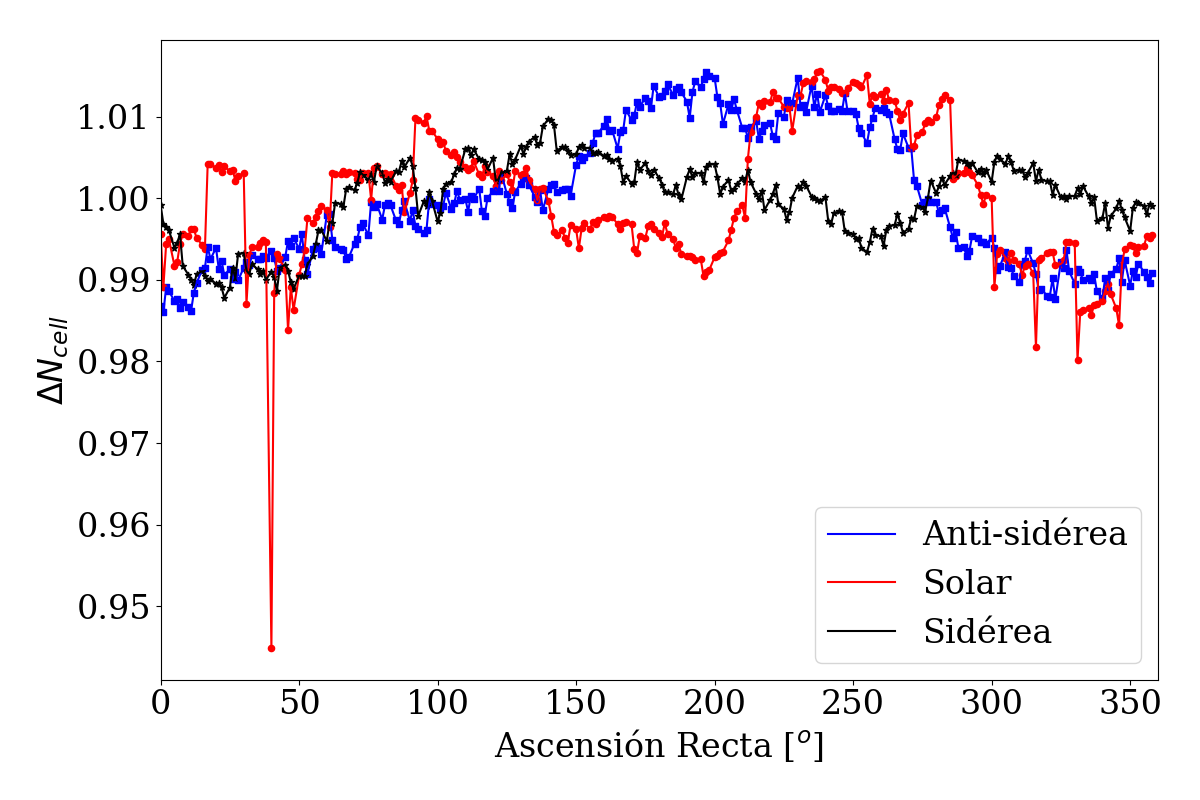
\includegraphics[width=0.8\textwidth]{weights_2013_2020.png}
				\caption{Variaciones de los hexágonos en función de la ascensión recta del observatorio para frecuencias características en rango mencionado. }
				\label{pesos_bin_1_2}
			\end{figure}


\section{Análisis de la modulación en ascensión recta para el primer armónico}

En la Fig.\ref{anisotropia_rayleigh} se muestra en barrido de frecuencias para la amplitud del primer armónico de Fourier. Se marcan con líneas verticales las frecuencias de referencia mencionadas anteriormente. Se observa el barrido sin considerar las correcciones por las variaciones de los hexágonos con una línea discontinua. La  amplitud  en la frecuencia solar sin la corrección de los pesos es importante. Un ejemplo de errores sistemáticos puede ser que en épocas invernales el acceso a los tanques se dificulta y ponerlos en funcionamiento nuevamente tras una tormenta o para un cambio de baterías puede llevar más tiempo que durante verano. 

		\begin{figure}[H]
			\centering
			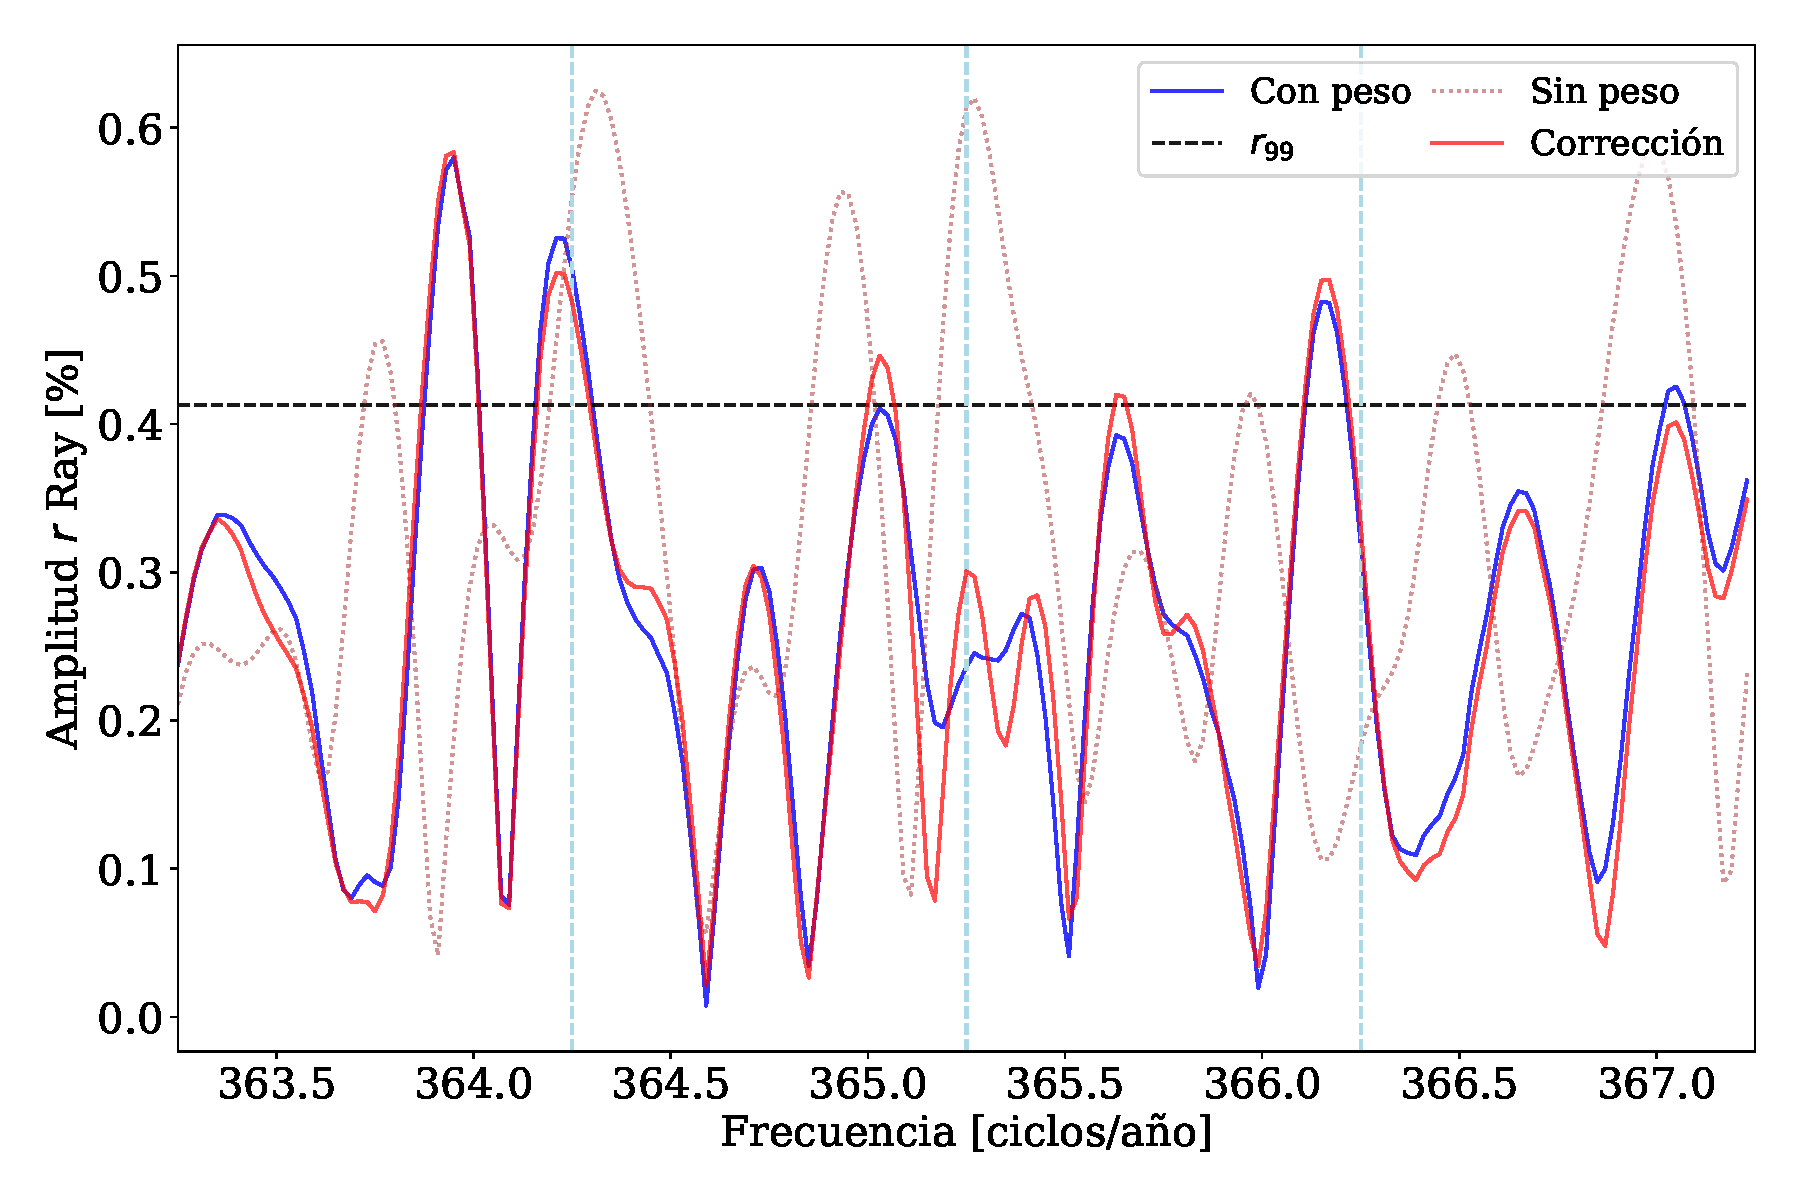
\includegraphics[width=0.75\linewidth]{pesos_sin_con_1_2_EeV.pdf}
			\caption{Anisotropía en función de la frecuencia para el rango de energía 1  EeV - 2 EeV. Se comparan los análisis sin los pesos y con los pesos de los hexágonos entre en 1 de Enero del 2014 y el 1 de Enero del 2020}
			\label{anisotropia_rayleigh}
		\end{figure}

Cuando se consideran los pesos, que se muestran con una línea azul en la Fig. \ref{anisotropia_rayleigh}, la amplitud de la frecuencia solar disminuye y pasa a estar por debajo del umbral de $r_{99}$, y aparecen dos amplitudes por encima de este umbral: un pico es la frecuencia sidérea, donde buscamos las anisotropías en ascensión recta, y otro pico es cerca de la frecuencia anti-sidérea, que indica que existen componentes de errores sistemáticos sobre los datos que deben ser considerados. 

Para disminuir las posibles modulaciones debidas a errores sistemáticos, se corrigió la modulación del clima de la  señal de $S_{38}$ de cada evento y se obtuvo la energía corregida con los parámetros de la sección \ref{ALL_modulacion}. El barrido de frecuencias sobre estos eventos se muestra en la Fig.\,\ref{anisotropia_rayleigh} con una línea roja continua. Se observa que disminuye ligeramente la amplitud en frecuencia anti-sidérea, pero aumenta en las frecuencias solar y sidérea.

% Por ejemplo, la corrección de clima que se analiza en el trabajo de licenciatura se realiza sobre el disparo estándar, se podría calcular los parámetros del clima utilizando los eventos de todos los disparos y comprobar si esto disminuye la amplitud del primer armónico de la frecuencia cercana a la anti-sidérea.

		
En la Tabla\,\ref{table:parametros_rayleigh} se resumen las amplitudes y fases obtenidas mediante el análisis a primer orden en Fourier en las frecuencias de referencia  y en la Tabla\,\ref{table:parametros_rayleigh_correccion} se reportan los valores de las mismas variables tras la corrección del clima utilizando los parámetros del capítulo anterior.
		\begin{table}[H]
		\centering
		\begin{tabular}{rc|c|c|}
			\cline{2-4}
			\multicolumn{1}{r|}{} & \multicolumn{3}{c|}{Sin pesos} 							 \\ \hline
			\multicolumn{1}{|l|}{Frecuencia:   }    & Anti-sidérea          & Solar          				& Sidérea     	 \\ \hline
			\multicolumn{1}{|l|}{Amplitud $r$[\%]:} & $0.55^{+0.15}_{-0.12}$& $0.61^{+0.15}_{-0.12}$        & $0.18^{+0.15}_{-0.08}$ \\
			\multicolumn{1}{|l|}{$r_{99}$ [\%]:   } & 0.41                  & 0.41                          & 0.41       \\
			\multicolumn{1}{|l|}{$r_{UL}$ [\%]:   } & 0.88                  & 0.95                          & 0.53       \\
			\multicolumn{1}{|l|}{$\sigma$:        } & 0.14                  & 0.14                          & 0.14          \\\hline
			\multicolumn{1}{|l|}{Probabilidad:    } & 0.0088                & $3.8\times 10^{-5}$                          & 0.40          \\
			\multicolumn{1}{|l|}{Fase [$^o$]:            } & 197$\pm$15            & 251$\pm$2                    & 289$\pm$47    \\\hline \\   \cline{2-4}
			
			\multicolumn{1}{r|}{} & \multicolumn{3}{c|}{Con pesos de los hexágonos} \\ \hline
			\multicolumn{1}{|l|}{Frecuencia:      } & Anti-sidérea          & Solar        	 				& Sidérea        \\ \hline
			\multicolumn{1}{|l|}{Amplitud $r$[\%]:} & $0.50^{+0.1}_{-0.12}$& $0.24^{+0.16}_{-0.09}$        & $0.32^{+0.16}_{-0.10}$ \\
			\multicolumn{1}{|l|}{$r_{99}$ [\%]:   } & 0.41                  & 0.41                          & 0.41       \\
			\multicolumn{1}{|l|}{$r_{UL}$ [\%]:   } & 0.84                  & 0.58                          & 0.66       \\
			\multicolumn{1}{|l|}{$\sigma$:        } & 0.14                  & 0.14                          & 0.14          \\\hline
			\multicolumn{1}{|l|}{Probabilidad:    } & 0.0010                & 0.22                          & 0.063          \\
			\multicolumn{1}{|l|}{Fase [$^o$]:            } & 85$\pm$16             & 260$\pm$5                    & 357$\pm$26    \\\hline 		
		\end{tabular}
		\caption{Comparación de los parámetros de fase y amplitud para las frecuencias anti-sidérea, sidérea y solar obtenidos de Todos los Disparos. Se analizaron estos parámetros sin pesos y con los pesos de los hexágonos con el análisis de Rayleigh entre en 1 de Enero del 2014 y el 1 de Enero del 2020}
		\label{table:parametros_rayleigh}
		\end{table}

		\begin{table}[H]
			\centering
			\begin{tabular}{rc|c|c|}
				\cline{2-4}
				\multicolumn{1}{r|}{} & \multicolumn{3}{c|}{Corregido por este  trabajo} \\ \hline
				\multicolumn{1}{|l|}{Frecuencia:      } & Anti-sidérea          & Solar        	 				& Sidérea        \\ \hline
				\multicolumn{1}{|l|}{Amplitud $r$[\%]:} & $0.48^{+0.15}_{-0.11}$& $0.30^{+0.16}_{-0.10}$        & $0.33^{+0.15}_{-0.11}$ \\
				\multicolumn{1}{|l|}{$r_{99}$ [\%]:   } & 0.42                  & 0.42                          & 0.42       \\
				\multicolumn{1}{|l|}{$r_{UL}$ [\%]:   } & 0.81                  & 0.64                          & 0.67       \\
				\multicolumn{1}{|l|}{$\sigma$:        } & 0.14                  & 0.14                          & 0.13          \\\hline
				\multicolumn{1}{|l|}{Probabilidad:    } & 0.0020                  & 0.089                       & 0.052          \\
				\multicolumn{1}{|l|}{Fase [$^o$]:            } & 85$\pm$17            & 204$\pm$5                    	& 354$\pm$25    \\\hline 
			\end{tabular}
			\caption{Comparación de los parámetros de fase y amplitud para las frecuencias anti-sidérea, sidérea y solar obtenidos de la señal corregida  de los  Todos los Disparos mediante los parámetros obtenidos en la sección \ref{ALL_modulacion}.}
			\label{table:parametros_rayleigh_correccion}
			\end{table}
	
\subsection{Tasa de eventos por ascensión recta}

Las Fig.\,\ref{fig:bin_events_first_order} se muestra la tasa de eventos normalizada con pesos y sin pesos para este rango de energía. Las líneas discontinuas representan los parámetros de la Tabla\,\ref{table:parametros_rayleigh} para el primer armónico del análisis de Rayleigh de la frecuencia sidérea. Se observa que la modulación de los eventos con y sin pesos tiene características que la aproximación a primer orden no refleja. 	
	\begin{figure}[H]
		\centering
		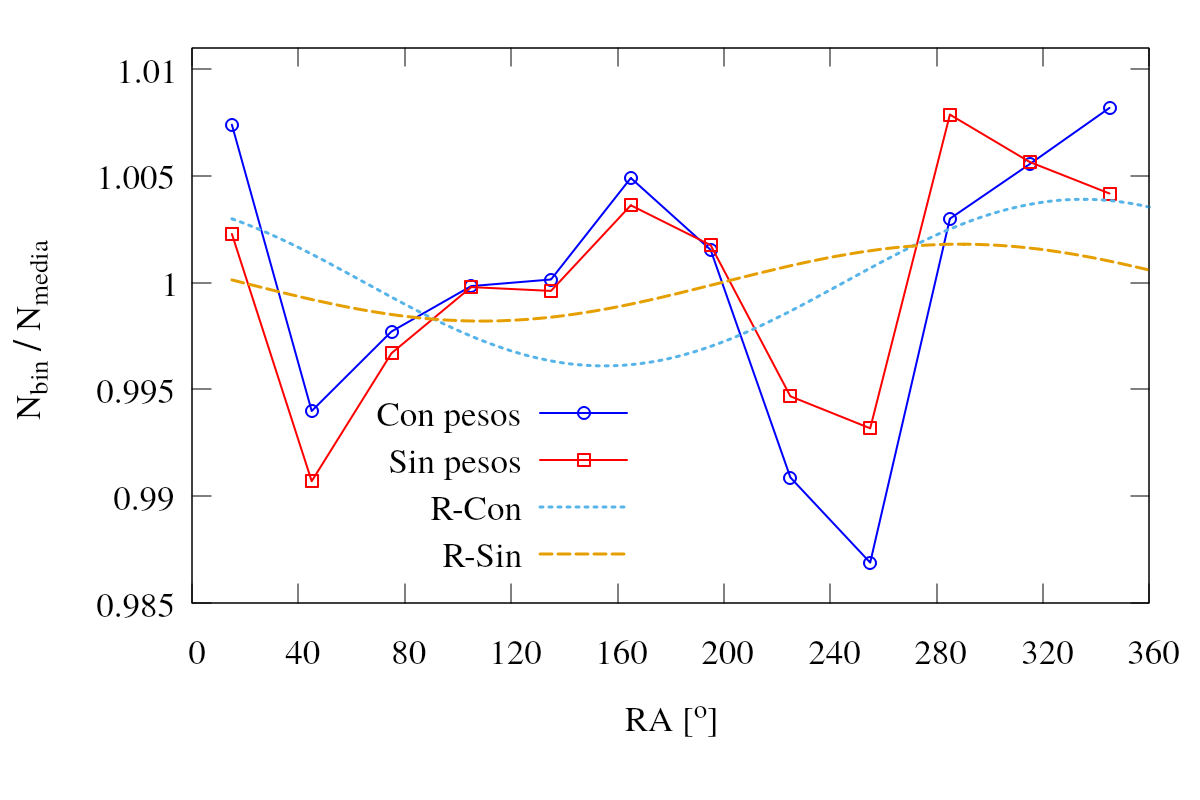
\includegraphics[width=0.8\linewidth]{eventos_clasificados_por_RA_v4.png}
		\caption{Distribución de la cantidad relativa de eventos en función de la ascensión recta a primer orden, en el rango de energía $1$ EeV - $2$ EeV.}
		\label{fig:bin_events_first_order}
	\end{figure}

\subsection{Análisis de segundo orden en Fourier}
	En las Fig.\,\ref{fig:bin_events_second_order_con} se muestra la tasa de eventos con pesos y el ajuste hasta el segundo orden en Fourier, en el mismo se muestra que este orden refleja mejor las características de los datos. Los resultados del análisis de Rayleigh  se muestran en la Tabla\,\ref{table:parametros_second_order}
        \begin{figure}[H]
          \centering
            \begin{subfigure}[b]{0.8\textwidth}
		\centering
		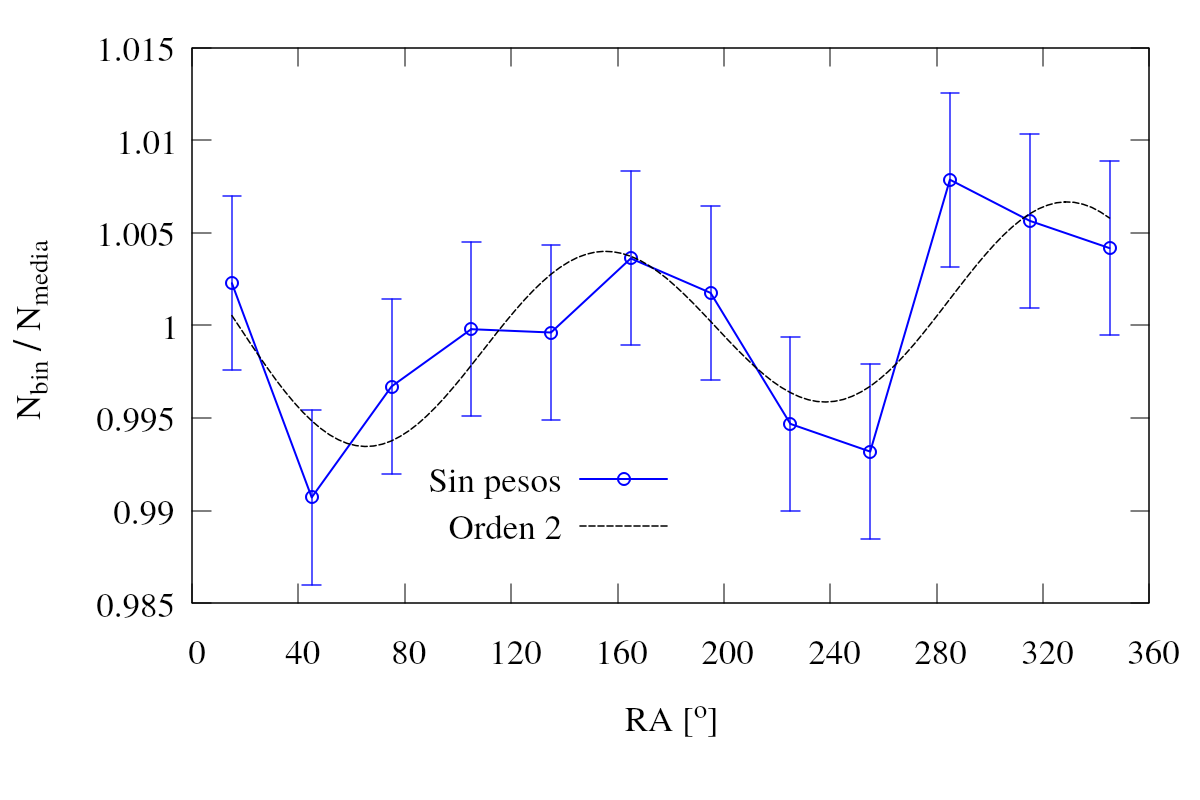
\includegraphics[width=\linewidth]{eventos_clasificados_por_RA_v7_orden_2_sin_pesos.png}
		\caption{Eventos sin pesos}		\label{fig:bin_events_second_order_sin}
            \end{subfigure}\\
            \begin{subfigure}[b]{0.8\textwidth}
		\centering
		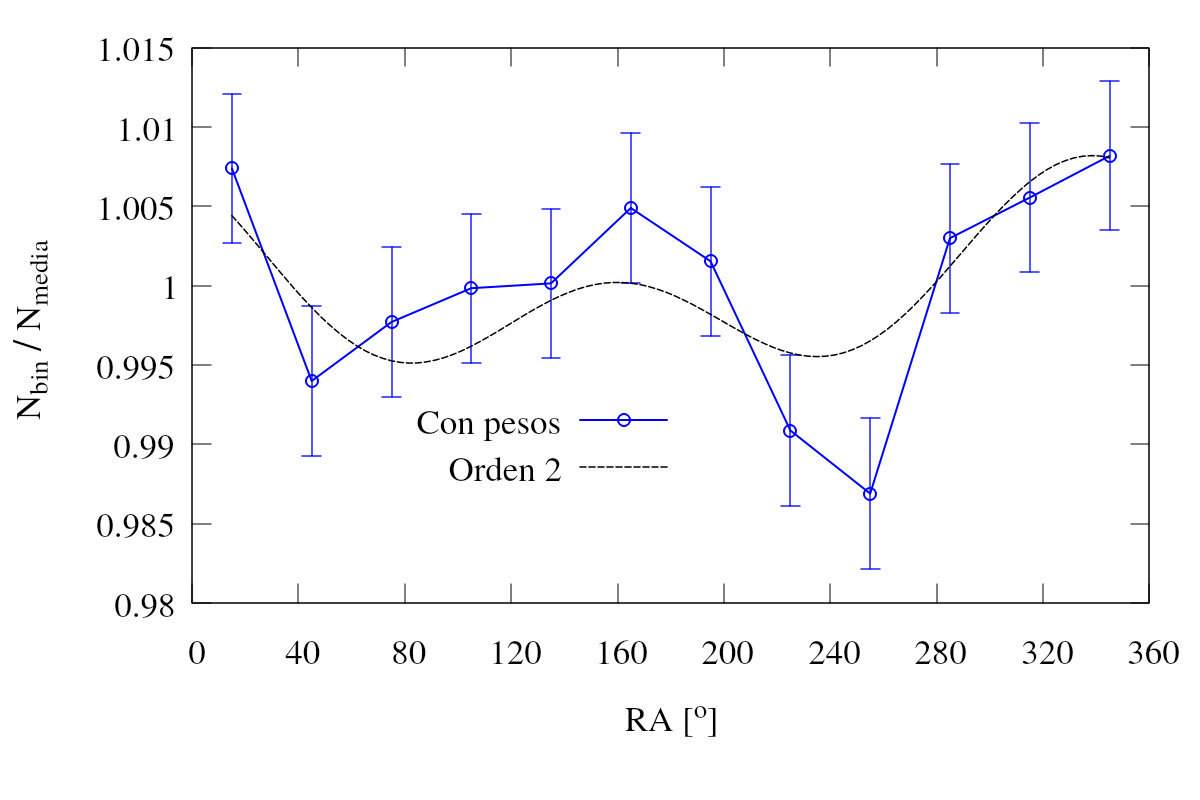
\includegraphics[width=\linewidth]{eventos_clasificados_por_RA_v7_orden_2_con_pesos.png}
		\caption{ Eventos con sus respectivos pesos}		\label{fig:bin_events_second_order_con}
            \end{subfigure}
           \caption{Distribución de la cantidad relativa de eventos en función de la ascensión recta a segundo orden en el rango de energía $1$ EeV - $2$ EeV entre en 1 de Enero del 2014 y el 1 de Enero del 2020.}
         \end{figure}

		\begin{table}[H]
		\centering
			\begin{tabular}{l|l|l|}
			\cline{2-3}
			                                      			& Sin Pesos 				 & Con Pesos \\ \hline
			\multicolumn{1}{|l|}{Orden k :}       			& 2                			& 2                    \\ \hline
			\multicolumn{1}{|l|}{Fase $\phi_2$ [$^o$]:}  	& $153\pm15$    				& $145\pm21$                   \\ \hline
			\multicolumn{1}{|l|}{Amplitud $r_2$ [\%]:} 		& $0.54^{+0.15}_{-0.12}$	& $0.38^{+0.15}_{-0.11}$               \\ \hline
			\multicolumn{1}{|l|}{Probabilidad $P(r_2)$:}    & $3.9\times 10^{-4}$\      & $0.017$  \\ \hline
			\end{tabular}
		\caption{Parámetros obtenidos del ajuste a segundo orden en ascensión recta con el análisis de Rayleigh.}
		\label{table:parametros_second_order}
		\end{table}
